\section{Lagrange points analysis}

Lagrangian points are a set of special locations in the vicinity of two massive
bodies where a small object will maintain a relatively stable position relative
to the two massive bodies. The five Lagrange points are labeled L1 through L5.
L1, L2, and L3 are collinear with the two massive bodies, while L4 and L5 are
located at the vertices of the equilateral triangle formed by the two massive
bodies. The L1, L2, and L3 points are unstable, while L4 and L5 are stable. The
L4 and L5 points are sometimes called Trojan points, and the two massive bodies
are sometimes called the primaries.

Despite L1, L2, and L3 being unstable, they are of particular interest because
of their proximity to the primaries. In fact, stable orbits can be achieved
by performing small corrections to the spacecrafts's position. Also, these
points are not populated with asteroids like L4 and L5, making them excellent
for long term missions.

In this work, only the point L2 belonging to the Sun - Earth system is
considered. The reason for choosing this point is that it is a popular point
chosed by different missions and thus, a well known point. It provides a great
viewpoint. In fact, this point has been selected for other missions including
the James Webb Space Telescope, see \cite{gardner2006}, or the future Comet
Interceptor, see \cite{jones2019}.

\begin{figure}[H]
    \centering
    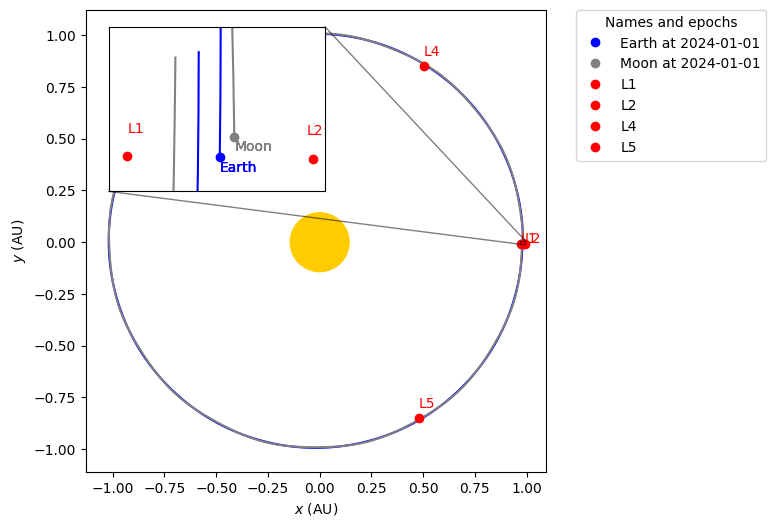
\includegraphics[width=\textwidth]{static/lagrange_points.png}
    \caption[Lagrange points in the Sun - Earth system.]{Lagrange points in the
        Sun - Earth system. All points are shown except L3. Ephemerides for this
        point are not provided by the JPL Horizons system. Despite this
        situation, the point is not analyzed in this work.}
    \label{fig:lagrange_points}
\end{figure}
